
\documentclass[preprint,12pt]{elsarticle}

\usepackage[spanish]{babel}
\usepackage{amssymb}
\usepackage{graphicx}
\usepackage{lineno}
\usepackage[utf8]{inputenc}
\usepackage{url}
\usepackage{natbib}

\begin{document}
	
	\begin{frontmatter}

		\title{\huge  COMPARATIVA DE DOS METODOLOGÍAS DE CALIDAD DE SOFTWARE) }
		\author{Pacora Silva, Jorge Carlos				(2013000725)}
		\author{Quenaya Buiza, Jesús Alejandro			(20200)}
		\author{Torres Beltran , Johanna Andrea			(2020067849)}
		\address{Tacna, Perú}
		


%%INICIO abstract
\begin{abstract}
Nowadays, the companies in charge of software development are prepared to cover a wide range of demand in this market, so their objective is to cover the needs of each client. However, problems in software development such as quality are still evident.
\\
This article describes the quality methodologies that are implemented to mitigate this problem. Since, the different methods are necessary for the accomplishment of the tests to which the software is put under to identify the quality of this product that is being given to the client.
However, it is necessary to emphasize that the technology advances, everything with respect to the components of the quality evolves simultaneously, with respect to which the classic quality was left aside that was shaped by means of a paper, to happen to the agile quality where new practices are implemented, where it is possible to conclude that in this evolution it is not only enough to have good lines of code and of course it is not paper, it goes beyond, where it is supported in scopes like the productivity, the happiness and the times of delivery of the projects.
\end{abstract}
%%FIN abstract


\end{frontmatter}

%%INICIO Resumen
\section{Resumen}
En la actualidad las empresas que se encargan del desarrollo de software están preparadas para cubrir amplia gama de demanda en este mercado, por lo que su  objetivo es cubrir las necesidades que cada cliente necesite. Sin embargo, aún se evidencian problemas en el desarrollo de software como lo es la calidad.
\\
\\
En el  presente artículo se describe las metodologías de calidad que son implementadas para mitigar este problema. Puesto que, los diferentes métodos  son necesarios para la realización de las  pruebas a las que es sometido el software para identificar la calidad de este producto que se le está entregando al cliente.
Sin embargo es necesario recalcar que a la tecnología avanza, todo respecto al los componentes de la calidad  evolucionan simultáneamente, respecto a que se dejó de un lado la calidad clásica que se plasmaba mediante un papel , para pasar a la calidad ágil donde se implementan nuevas prácticas, donde se puede concluir que en esta evolución no solo basta con tener buenas líneas de código y por supuesto no es papel, va más allá, donde se apoya en ámbitos como la productividad, la felicidad y a los tiempos de entrega de los proyectos.
%%FIN Resumen


%%INICIO Introducción
\section{Introducción}
xxxxxxxxxxxxxxxxxxxxxxxxxxxxxxxxxxxxxxxxxx
\\
\\
xxxxxxxxxxxxxxxxxxxxxxxxxxxxxxxxxxxxxxxxxxxxxxxxxxxxxx
\\

%%FIN Introducción


%%INICIO Marco Teórico
\section{Marco Teórico}

%%----------------------------------------------------------------------------------------------------------------------------------------------------------
	\subsection{\textbf{Titulo de la primera medotologia}}
	Hay que tomar en cuenta que este concepto Business Intelligence es un tema que viene desde octubre de 1958 
por Hans Peter Luhn (Investigador de IBM). Este concepto ha evolucionado aunando diferentes tecnologías, metodologías
 y términos.\cite{referenciarobles1}
\\
\\
Según el glosario de términos de Gartner (2012) se extrae la siguiente definición:“BI es un proceso interactivo para explorar y analizar información estructurada sobre un área (normalmente almacenada en un “datawarehouse”), para descubrir tendencias o patrones, a partir de los cuales derivar ideas y extraer conclusiones. El proceso de BI incluye la comunicación de los descubrimientos y efectuar los cambios. Las áreas incluyen clientes, proveedores, productos, servicios y competidores.” \cite{referenciaestrella2}
\\
\\
Según Vitt (2002):
“El BI es usado por diferentes usuarios y desarrolladores de software para distinguir un amplio rango de tecnologías, plataformas de software, aplicaciones específicas y procesos. Se utiliza este término desde tres diferentes perspectivas:
	\begin{itemize}
	\item Tomar mejores decisiones rápidamente.
	\item Utilizar un método razonable para la gestión empresarial.”  \cite{referenciaestrella3} \\
	\end{itemize}

Business Intelligence  es un conjunto de metodologías, aplicaciones, prácticas y capacidades enfocadas a la creación
 y administración de información que permite tomar las mejores decisiones a los usuarios en una organización.

	\subsubsection{\textbf{Componentes de una Arquitectura de BI}}

	Los componentes son:

	\begin{itemize}
	\item Las herramientas de visualización, que nos permitirán el análisis y la navegación a través de los mismos. \cite{referenciaestrella3}

	\end{itemize}

\begin{figure}[htb]
	\begin{center}
		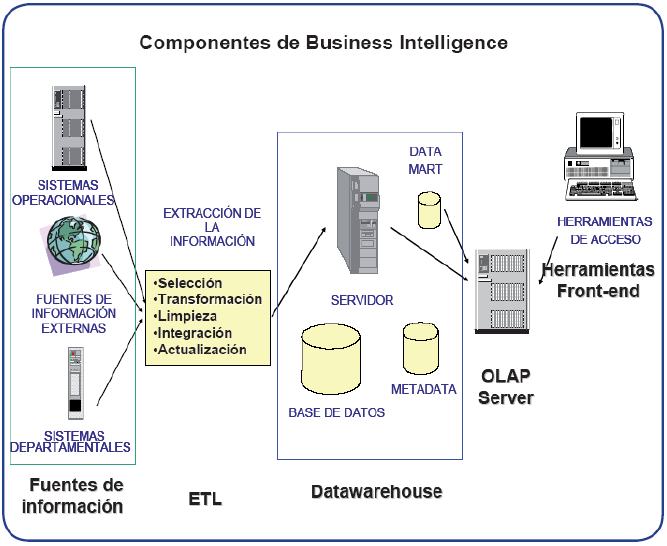
\includegraphics[width=14cm]{./IMAGENES/componentes} 
		\caption{Componentes de Business Intelligence}
	\end{center}
\end{figure}

%%****

\subsubsection{\textbf{xxxxxxxxxxxxxxxx}}

La Inteligencia de Negocios en una plataforma de administración del desempeño que representa al ciclo en el que las empresas establecen sus objetivos, analizan sus progresos, reflexionan, actúan, miden su éxito y empiezan una nueva fase. \\ \\Su ciclo se compone de cuatro etapas a saber: Análisis, reflexión, acción y medición. \cite{referenciaestrella1}

\begin{figure}[htb]
	\begin{center}
		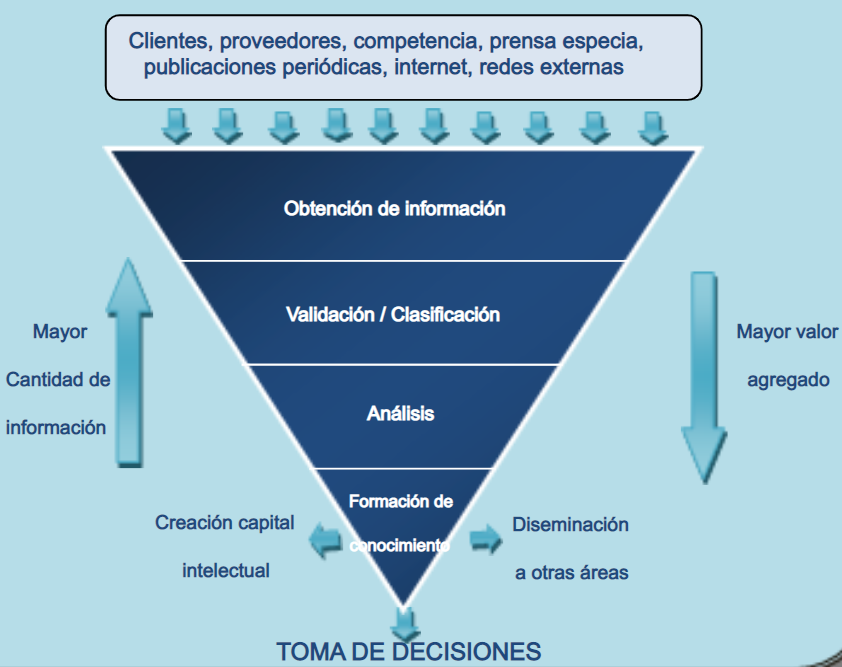
\includegraphics[width=12cm]{./IMAGENES/ciclo_BI} 
		\caption{Ciclo de Inteligencia de Negocios}
	\end{center}
\end{figure}

%%****
	\subsubsection{\textbf{Beneficios de un sistema de Inteligencia de Negocio (BI)}}
	La implantación de estos sistemas de información proporciona diversos beneficios entre los que podemos destacar:

	\begin{itemize}
	\item xxxxxxxxxxxxxxxxxxxxxxxxxxxxxxxxxxxxxxxxxxxxxxxxxxxxxxxxxxxxxxxxxx.
	\item xxxxxxxxxxxxxxxxxxxxxxxxxxxxxxxxxxxxxxxxxxxxxxxxxxxxxxxxxxxxxxxxxxxxxxxxxxxxxxxxxxxxxx.
	\end{itemize}\cite{referenciarobles3}
%%****
	\subsubsection{\textbf{La necesidad de la Inteligencia de Negocio}}
	Existen situaciones en las que la implantación de un sistema Business Intelligence  resulta adecuada. Podríamos destacar 
	entre las que existen son:

	\begin{itemize}
	\item xxxxxxxxxxxxxxxxxxxxxxxxxxxxxxxxxxxxxxxxxx
	\item Lxxxxxxxxxxxxxxxxxxxxxxxxxxxxxxxxxxxxxxxxxxxxxxxxxxxxxxx

	\end{itemize}

%%****
	\subsubsection{\textbf{xxxxxxxxxxxxxxxxxxxxxxxxxxxxxxx}}
	Desplegar un proyecto de inteligencia de negocio en una organización no es un proceso sencillo. Las buenas practicas dicen 
	que para llegar a un buen puerto, es necesario tener una estrategia de inteligencia de negocio que coordine de forma efectiva 
	las tecnologías, el uso, los procesos de madurez.\cite{referenciarobles2}
%%****
	\subsubsection{\textbf{xxxxxxxxxxxxxxxxxxxxxxxxxxxxxxx}}
	xxxxxxxxxxxxxxxxxxxxxxxxxxxxxxxxxxxxxxxxxxxxxxxxxxxxxxxxxxxxxxxxxxxxxs:

	\begin{itemize}
	\item xxxxxxxxxxxxxxxxxxxxxxxxxxxxxxxxxxxxxxxxxxxxxxxxxxxxxxxxxxxxxxxxxxx
	\end{itemize}


%%****
	\subsubsection{\textbf{xxxxxxxxxxxxxxxxxxxxxxxxxxx}}
	xxxxxxxxxxxxxxxxxxxxxxxxxxxxxxxxxxxxxxxxxxxxxxxxxx:

	\begin{itemize}
	\item xxxxxxxxxxxxxxxxxxxxxxxxxxxxxxxxxxxxxxxxxxxxxxxxxxxxxxxxxxxxxxxxxxxxxxxxxxxxxxxx
	\item  xxxxxxxxxxxxxxxxxxxxxxxxxxxxxxxxxxxxxxxxxxxx
	
	\end{itemize}



%%-----------------------------------------------------------------------------
	\subsection{\textbf{Analítica de Negocios (BA) }}
	Business Analytics son un conjunto de tecnologías que ayudan a los usuarios a analizar grandes datos empresariales para tomar decisiones mejores y más efectivas. \\\\
Es una colección de habilidades, tecnologías, aplicaciones y prácticas para la investigación continua y repetitiva de los datos, y así poder explicar el desempeño empresarial histórico, actual y futuro\cite{referenciasosa1}.\\
\\Al estudiar estos datos, las empresas pueden responder preguntas como“¿Qué está pasando?”, “¿Por qué está sucediendo?” Y “¿Qué va a pasar?”\cite{referenciasosa3}, también determinar los mejores modelos y enfoques analíticos, descubriendo las oportunidades actuales y tendencias futuras acerca de los clientes en relacón con su producto/servicio, y así presentar estas soluciones, a los usuarios empresariales, que permitirán a la organización alcanzar sus objetivos estratégicos.\\
Schnierderjans et al.(2014) en su libro resumieron que el BA incluye los mismos procedimientos que en la analítica simple, pero tiene el requisito adicional de que el resultado del análisis analítico debe tener un impacto medible en el rendimiento de la empresa. \cite{referenciasosa2} \\
\\Simplemente, los análisis convierten los datos en información útil para la empresa.

	\subsubsection{\textbf{Tipos l}}
	\begin{itemize}
	\item{\textbf{1. Análisis descriptivo:}}xxxxxxxxxxxxxxxxxxxxxxxxxxxxxxxxxxxxxxxxxxxxxxx	
	\item {\textbf{2. Análisis  predictivo:}}xxxxxxxxxxxxxxxxxxxxxxxxxxxxxxxxxxxxxxx
	\item {\textbf{3. Análisis prescriptivo:}}xxxxxxxxxxxxxxxxxxxxxxxxxxxxxxxxxxxx
	\end{itemize}

	\subsubsection{\textbf{BA Framework }}
El marco general de BA incluye cuatro capas: capa de datos, capa de análisis, capa de información / visualización y capa de acceso.
Estas capas se analizan a continuación\cite{referenciasosa1}: 
\begin{figure}[htb]
	\begin{center}
		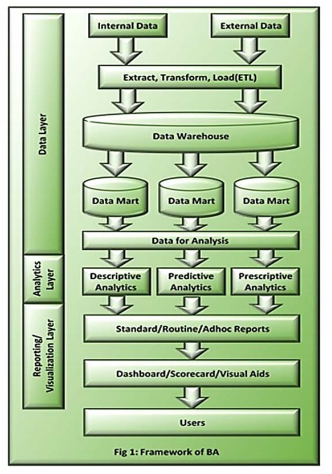
\includegraphics[height=10cm]{./IMAGENES/BAFramework} 
		\caption{Framework de BA}
	\end{center}
\end{figure}

	\begin{itemize}
	\item \textbf{Capa de datos:} se recopilan los datos de fuentes internas y externas. Las fuentes de datos internas incluyen
	Algunas herramientas utilizadas en la capa de datos se encuentran:
		\begin{itemize}
		\item xxxxxxxxxxxxxxxxxxxx
		\end{itemize}

	\item \textbf{Capa de Análisis:} En esta capa, los datos del Data Warehouse/DataMart se analizan mediante análisis descriptivos, predictivos y preceptivos.
		\begin{itemize}
		\item xxxxxxxxxxxxxxxxxxxxxxxxxxxxxxxxxxxxxxxxxxxxxxxxxxxxxxxxxxxxxxxxxxxxxxxxxxxxxxxxxxxxx
		\end{itemize}

		\item \textbf{Capa de Reportes y Visualización:} En esta capa se encuentran varias herramientas para poder visualizar la información analizada:
		\begin{itemize}
		\item Dashboard: son herramientas para visualizar datos comerciales importantes que se muestran en forma de indicadores gráficos, cuadros y tablas. \\Los paneles digitales ofrecen a los usuarios una vista gráfica avanzada de los procesos comerciales, que se puede subdividir para encontrar información más detallada sobre procesos comerciales específicos.
		\item xxxxxxxxxxxxxxxxxxxxxxxxxxxxxxxxxxxxxxxxxxxxxxxxxxxxxxxxxx
\begin{figure}[htb]
	\begin{center}
		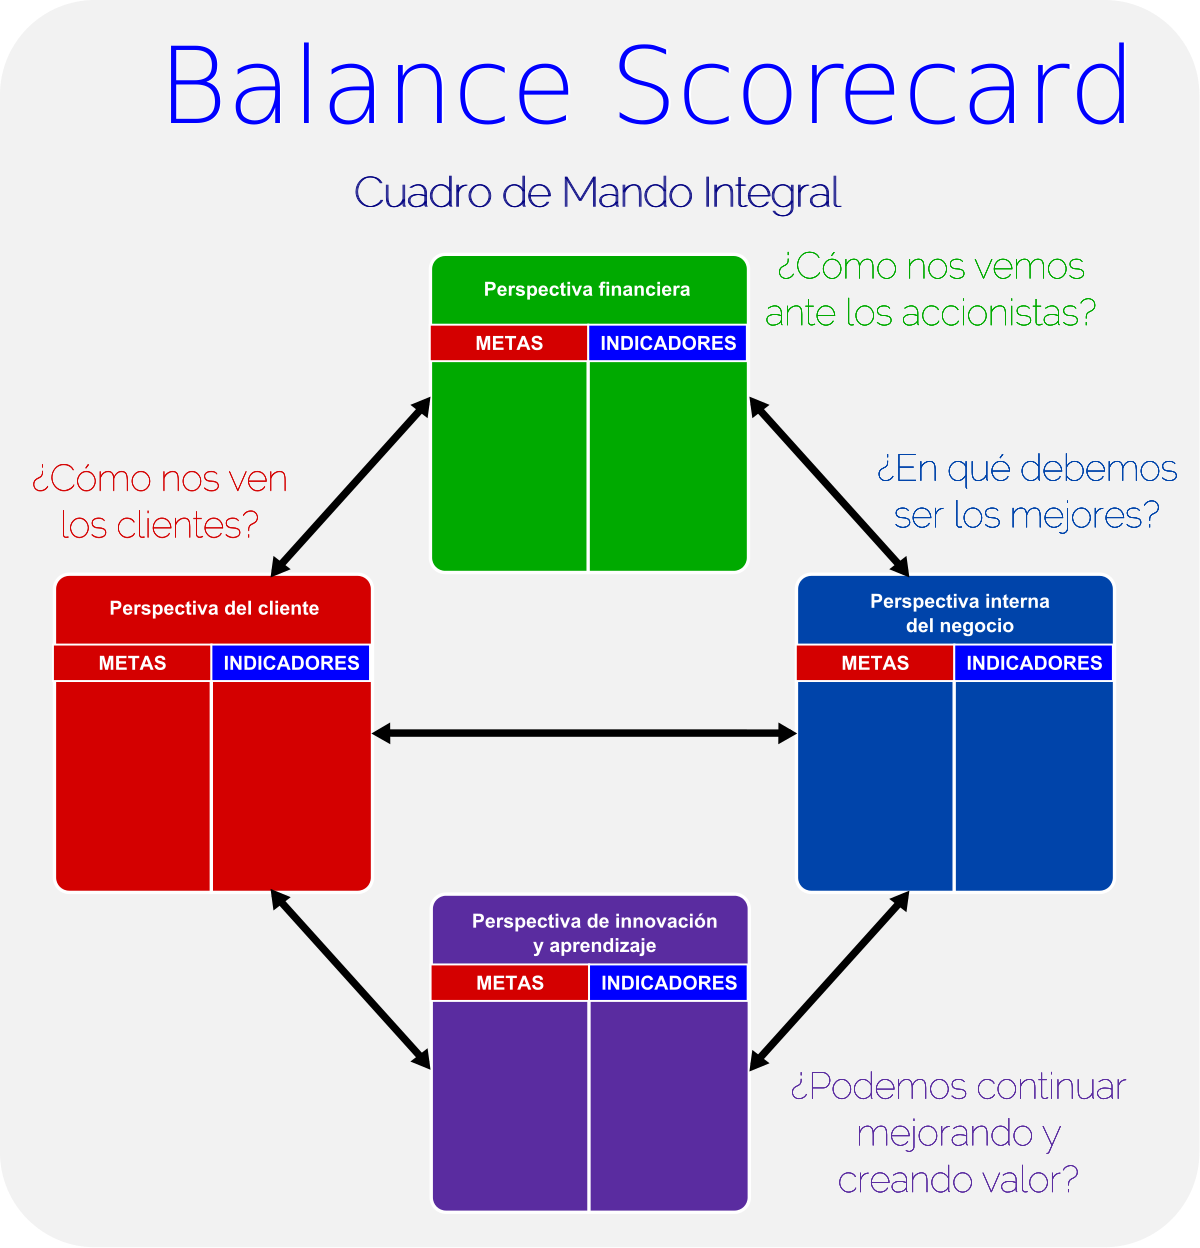
\includegraphics[width=7cm]{./IMAGENES/BalanceScorecard} 
		\caption{BalanceScorecard por Kaplan}
	\end{center}
\end{figure}

		\item Informes ad hoc: A diferencia de los informes estándar, que están predefinidos y se procesan de forma rutinaria, los informes ad hoc se generan cuando surge la necesidad. Permiten a los usuarios producir sus propios informes personalizados sin depender del equipo de TI.
		\end{itemize}

	\end{itemize}
\cite{referenciajohanna1}
%%-----------------------------------------------------------------------------

	

%%----------------------------------------------------------------------------------------------------------------------------------------------------------
%%FIN Marco Teórico

%COMPRACION

\section{Comparación entre  xxxxxxxxxxxxxxxxxxxxxxxxxx)}
A continuacion se muestra la comparación entre xxxxxxxxxxxxxxxxxxxxxxxxxxx:
	
	\begin{itemize}

	\item{\textbf{1.}} xxxxxxxxxxxxxxxxxxxxxxxxxxxxxxxxxxxxxxxxx.
	\item{\textbf{2.}} xxxxxxxxxxxxxxxxxxxxxxxxxxxxxxxxxxxxxxxxx.

\end{itemize}


%CONCLUSIONES
\section{Conclusiones}

%%****
	\begin{itemize}
\item xxxxxxxxxxxxxxxxxxxxxxxxxxxxxxxxxxxxxxxx
\item xxxxxxxxxxxxxxxxxxxxxxxxxxxxxxxxxxxxxxxxxxxxxxxxx
	\end{itemize}



%RECOMENDACIONES
\section{Recomendaciones}	
	\begin{itemize}

	\item Si una empresa está buscando entender de una mejor manera las operaciones internas, descubrir fallos en sus procesos, identificar posibles indicadores, probablemente necesite una solución de BI y si quiere predecir los comportamientos futuros de sus clientes y de su negocio para adaptarse rápidamente al cambio y mejorar continuamente, probablemente necesite una solución de BA.
	\end{itemize}

	
	\newpage
	\bibliographystyle{apalike}
	\bibliography{BIBLIOGRAFIA}	
%\citep{referenciarobles2}  


% https://revistas.udistrital.edu.co/index.php/tia/article/view/4639/7094
% http://revistas.unitru.edu.pe/index.php/PGM/article/view/193/199
% http://www.spentamexico.org/v4-n2/4(2)%2016-52.pdf          ---> PAGINA 18


\end{document}

